\subsection{Spider evaluation with GPT 3.5 and GPT 4}

Throughout this thesis, we have explored the advancements in Text-to-SQL models and their performance on the SPIDER benchmark. Our analysis revealed the significant progress made in the field, with more recent models demonstrating remarkable improvements in generating accurate SQL queries from natural language text.

The integration of powerful pre-trained language models, such as BERT, and cutting-edge architectures like T5 has played a vital role in the observed advancements. The models' ability to learn from limited labeled data, quickly adapt to new tasks or domains, and handle complex SQL queries has been substantially enhanced by employing techniques such as active learning, meta-learning, and multi-task learning.

Our experiments with ChatGPT-3.5 and ChatGPT-4.0 have showcased their superior performance, achieving scores of 81.30\% and 85.20\% on the SPIDER benchmark, respectively. These results highlight the potential of utilizing the latest huge language models for Text-to-SQL tasks, further pushing the boundaries of what is possible in this domain.

As the field of natural language processing continues to evolve, we can expect even more sophisticated models and techniques to emerge, enabling more accurate and efficient understanding and generation of SQL queries from natural language input. Future research in this area may focus on enhancing the models' ability to handle ambiguous or imprecise input, as well as exploring novel methods to improve their adaptability and generalization capabilities across diverse tasks and domains.

\begin{table}[H]
    \centering
    \begin{tabular}{|c|c|c|c|c|c|}
        \hline
        \multirow{2}*{Accuracy} & easy  & medium & hard  & extra hard & all            \\
                                            & 248   & 446    & 174   & 166        & 1034           \\ \hline
        GPT 3.5 execution                   & 0.964 & 0.883  & 0.644 & 0.596      & 0.816          \\ \hline
        GPT 3.5 exact match                 & 0.972 & 0.881  & 0.621 & 0.596      & 0.813          \\ \hline
        GPT 4 execution                     & 0.980 & 0.930  & 0.678 & 0.651      & \textbf{0.855} \\ \hline
        GPT 4 exact match                   & 0.980 & 0.933  & 0.667 & 0.639      & \textbf{0.852} \\ \hline
    \end{tabular}
    \caption{Comparison between Accuracies}
\end{table}

In conclusion, our experience using the ChatGPT API for the Text-to-SQL task on the SEOSS dataset was positive. The model's powerful natural language understanding capabilities, combined with the ease of integration through the API, make it a valuable tool for addressing such tasks. Additionally, by incorporating a few values from the database into the system input prompt, ChatGPT can better comprehend the database structure and generate more accurate queries. Also, by including the history of queries in prompts, we can improve the model's accuracy, but it will increase the overall time and money required to generate the queries. Future work could involve further fine-tuning ChatGPT specifically for Text-to-SQL tasks or exploring more advanced techniques for error correction and query validation.

% add SPIDER benchmark diagram image
\begin{figure}[H]
    \centering
    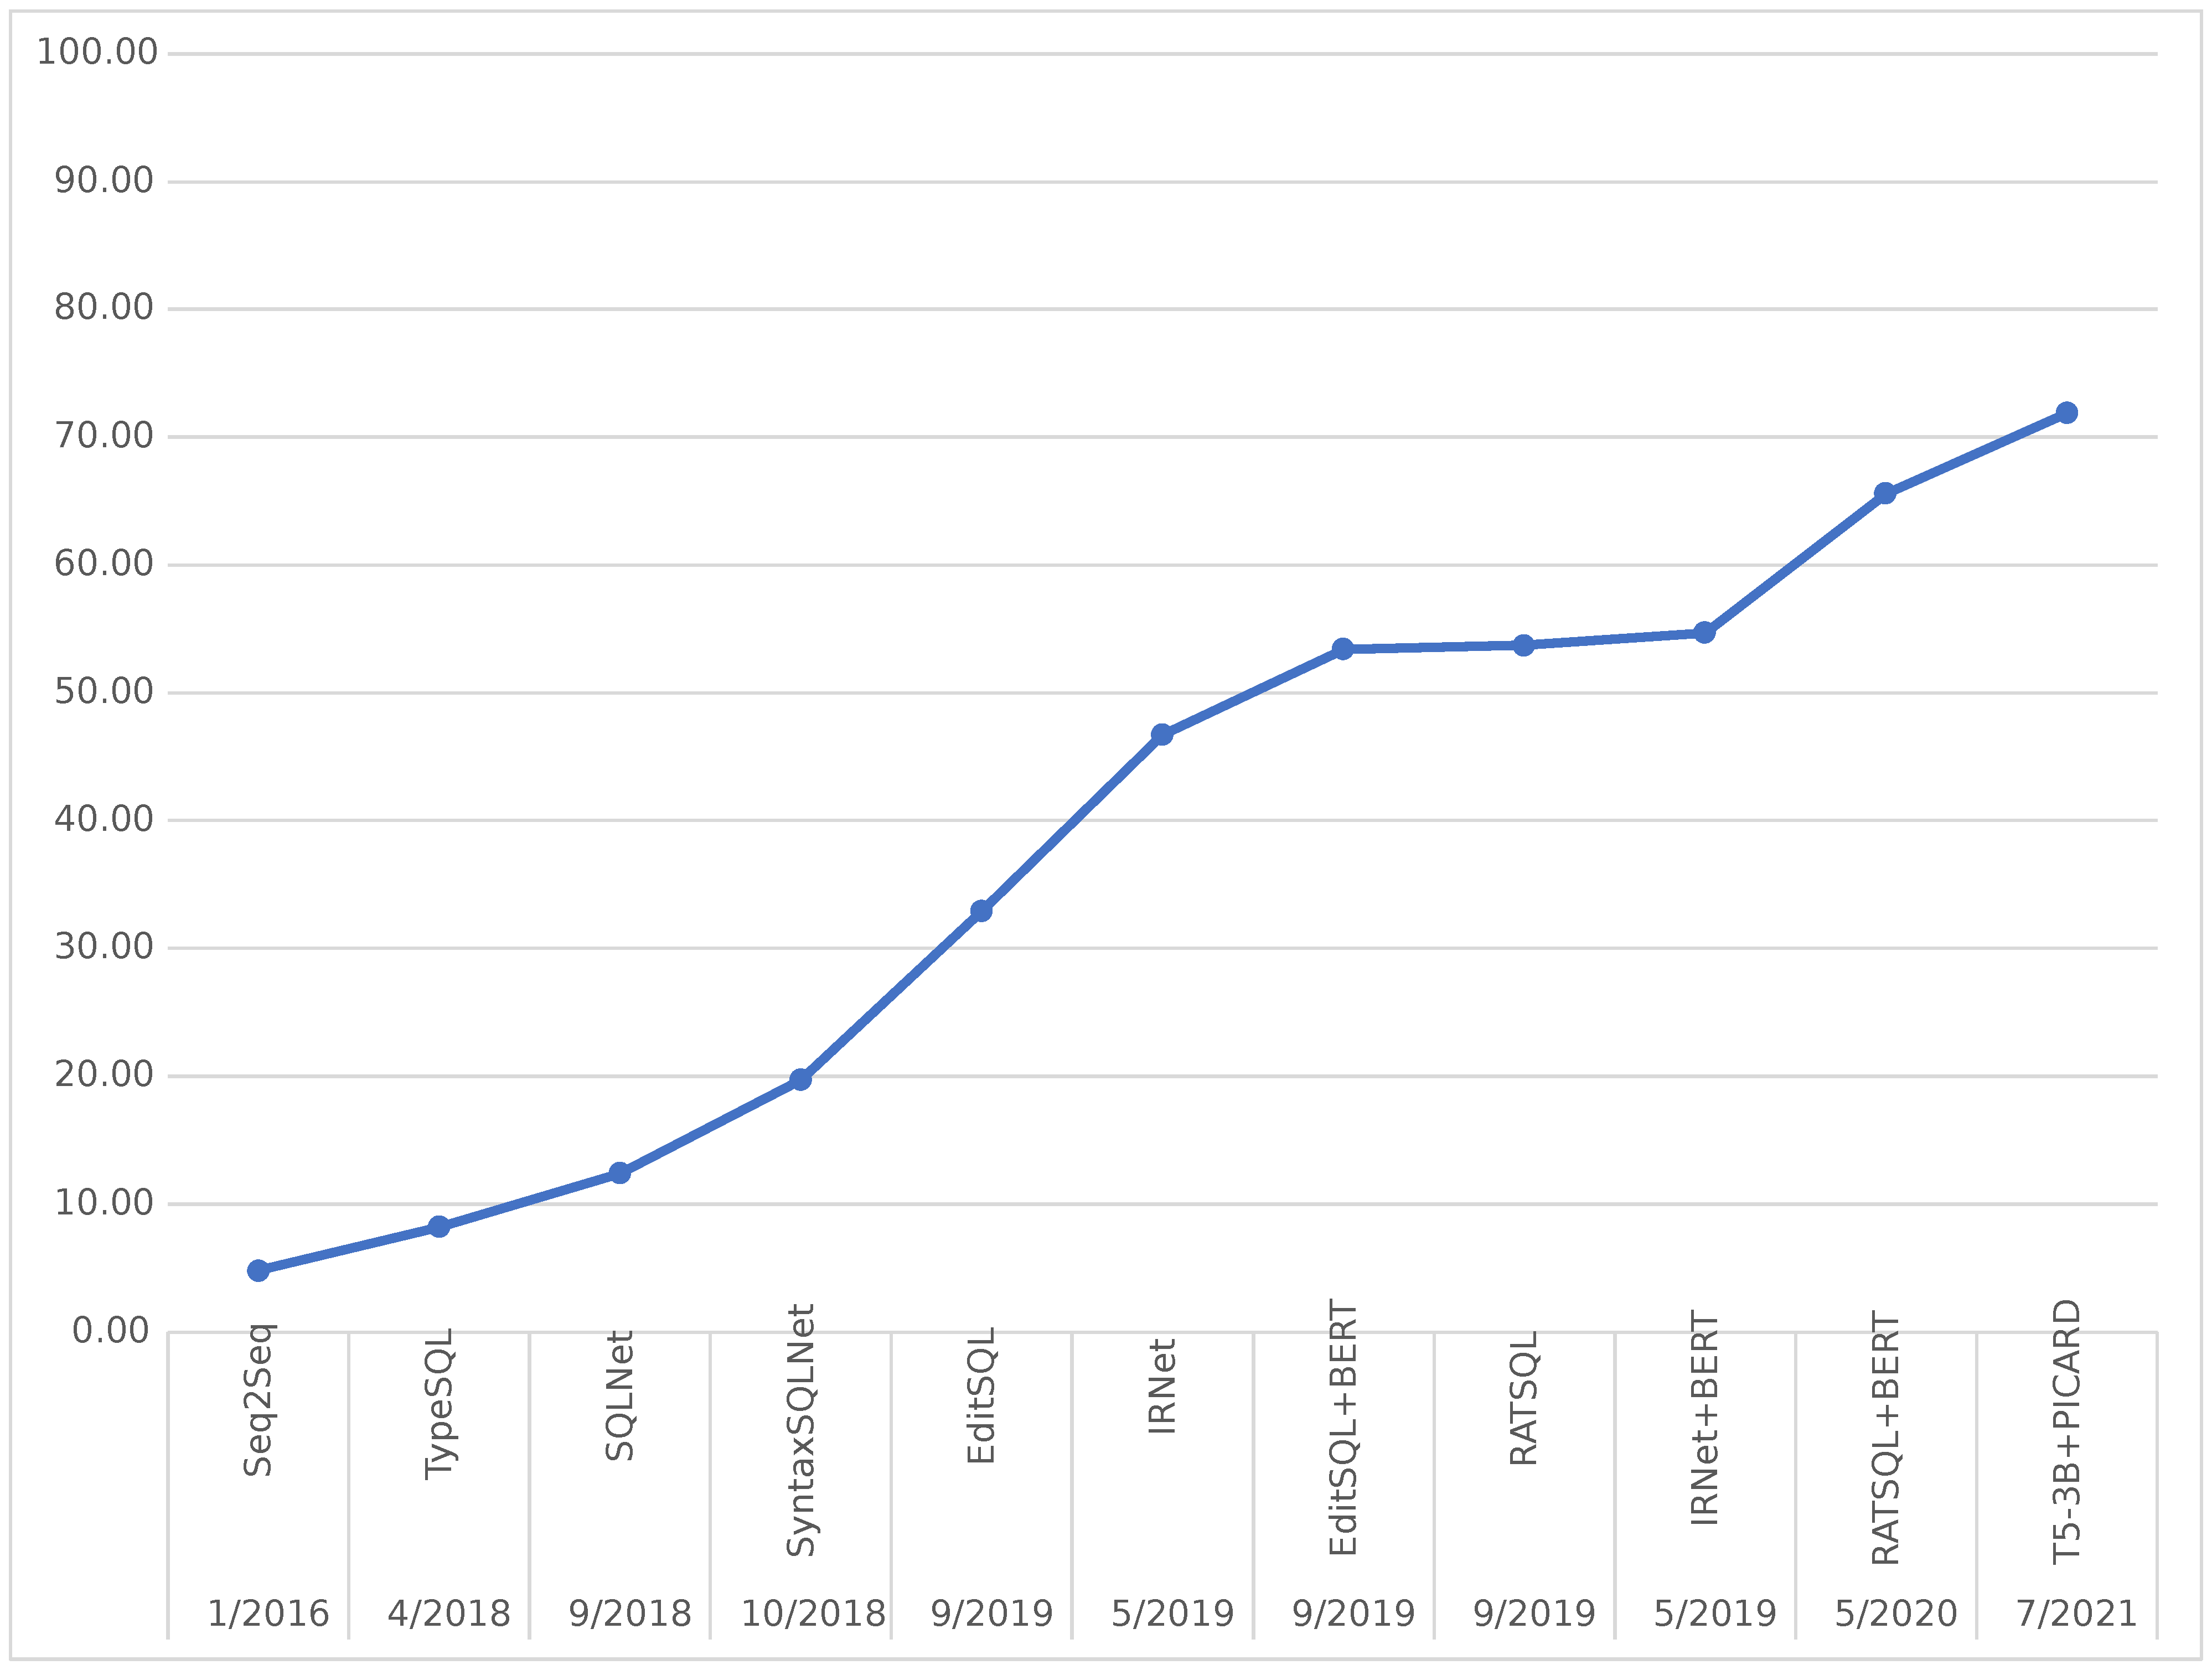
\includegraphics[width=0.99\linewidth]{pics/benchmarkeps}
    \caption{SPIDER benchmark Exact Match Results including our experiments}
    \label{fig:benchmark}
\end{figure}

\subsubsection{Cost Reduction}

We also compared the cost of running the queries generated by the different models. We found that the \ac{GPT} 4 model was the most expensive to run, followed by the GPT 3.5-turbo. This is because GPT 4 is a larger model requiring more resources. However, the GPT 4 model was also the most accurate, which means that it could generate more efficient queries requiring fewer resources to run. This is an important consideration when choosing a model for a production environment.

We can reduce the cost by minimizing the number of tokens we send to OpenAI API. We can do this by only giving the necessary information for the model to understand the task. Also, the number of tokens we receive from the model can be reduced by prompting the model to generate only the SQL query.

The other technique we used to reduce the cost was to use the GPT 3.5 turbo model to generate the SQL query, and for failed queries, we used the GPT 4 model to generate the SQL query. This technique reduced the cost significantly but nearly 45\%.

\subsubsection{Further Refinement}

In order to optimize the performance and precision of the model, various strategies can be implemented. These approaches focus on providing the model with more context and relevant information, which in turn enhances its ability to generate accurate SQL queries. The following sections outline two such methods that have proven to be effective in refining the model's output.

\subsubsubsection{Database Sample Integration}

A selection of brief examples was utilized within the prompt to enhance the precision of the produced SQL queries.

Employing an identical prompt configuration as the preceding one, several records from database tables, in conjunction with the database schema, may be incorporated to facilitate GPT's comprehension of the database's intricacies. This enabled the model to assimilate the information and generate increasingly precise SQL queries.

\subsubsubsection{Incorporating History and few shot examples}

The model's capacity to learn from prior queries or some examples was augmented, thus improving the generated SQL queries' accuracy.

By examining previous query outcomes and employing them within the prompt in the assistant capacity, the model's generation of increasingly precise SQL queries can be supported by presenting a historical record of actions. While implementing these refinement strategies, a potential increase in API costs is an important consideration. As the number of tokens per request increases due to the inclusion of additional context and information, the cost associated with each API call will rise significantly. It is crucial to weigh the benefits of improved accuracy and precision against the increased expenditure and strike a balance that ensures optimal model performance and cost efficiency.

\begin{figure}[H]
    \begin{AIbox}{Example of a Prompt with History and Database Sample}
        \vspace{-5px}
        \parbox{1\textwidth}{\scriptsize
        \begin{alltt} \larger
            {\bf role(System):} \\ 
            You are a helpful text-to-sql assistant for generating syntactically correct read-only                   \\
            SQL to answer a given question.                                                              \\
            Database: concert\_singer                                                                         \\
            The following are tables you can query:                                                      \\
            ---------------------                                                                        \\
            table name: stadium  table columns: Stadium\_ID [number (13)], Location [text (LA)], Name [text (SLA)], Capacity [number (30000)], Highest [number (20000)], Lowest [number (100)], Average [number (1000)] table name: singer  table columns: Singer\_ID [number (1)], NName [text (John Doe)],Country [text (USA)],Song\_Name [text (Beautiful Day)],Song\_release\_year [text (2020)],Age [number (30)],Is\_male [others (Yes)]      table name: concert  table columns: concert\_ID [number (101)],concert\_Name [text (Rock Night)],Theme [text (Rock Music)],Stadium\_ID [text (13)],Year [text (2023)]      table name: singer\_in\_concert  table columns: concert\_ID [number (101)], Singer\_ID [text (1)]       \\
            ---------------------                                                                        \\
            Do not use IN keyword.                                                                       \\
            If it is necessary to use AS then use it like T1 T2 ..., but if the alias                    \\
            name is not going to be used in query again, then do not use.                                \\
            Do not filter WHERE for being NOT NULL if it is not necessary.                               \\
            If in using  COUNT(*) and COUNT(COLUMN) there is no difference then use COUNT(*). \\
            Write one valid SQL in markdown format.
            \\
            {\bf role(User):} \\
            Generate syntactically correct read-only SQL to answer the following question: How many singers do we have?
            \\
            {\bf role(Assistant):} \\
            SELECT count(*) FROM singer
            \\
            {\bf role(User):} \\
            Generate syntactically correct read-only SQL to answer the following question: What are the names, countries, and ages for every singer in descending order of age?
            \\
            {\bf role(Assistant):} \\
            SELECT name,  country,  age FROM singer ORDER BY age DESC
            \\
            {\bf role(User):} \\
            Generate syntactically correct read-only SQL to answer the following question: \$question
        \end{alltt}
        }
        \vspace{-5px}
    \end{AIbox}
    \captionsetup{font={scriptsize,color=white}, skip=-20pt}
    \caption{Example of a Prompt with History and Database Sample}
\end{figure}

\subsubsubsection{Retries and Feedback}

In certain situations, ChatGPT may generate incorrect or unsatisfactory outputs. To improve the model's performance, we have investigated several techniques involving retries and feedback. Our experiments have led to the following observations:

\textbf{Retry without modifications}: Asking ChatGPT to retry without providing any specific guidance or feedback rarely led to improved results. Even when repeating the process multiple times, there was no significant improvement in the quality of the outputs and ChatGPT will insist on the correctness of the output.

\textbf{Rephrasing the user's question}: Requesting the model to rephrase the user's question before attempting to generate an answer yielded better outcomes in some cases. This method proved helpful in easy and medium tasks, resulting in the generation of new and improved queries. However, this approach's effectiveness diminished after the first retry, with no further improvements observed.

\textbf{Human-guided feedback}: Incorporating a human agent's feedback to point out issues in the generated output and instructing ChatGPT to address the problem led to noticeable improvements. In our experiments, we provided feedback in the form of "This is wrong. \$reason," and ChatGPT made appropriate adjustments based on the given reason.

\begin{figure}[H]
    \begin{AIbox}{Example a Feedback Prompt}
        \vspace{-10px}
        \parbox{1\textwidth}{\scriptsize
        \begin{alltt} \larger
            {\bf role(User):} \\
            Show the stadium name and the number of concerts in each stadium.
            \\
            {\bf role(Assistant):} \\
            SELECT stadium.Name, COUNT(concert.concert\_ID) AS Num\_Concerts FROM stadium LEFT JOIN concert ON stadium.Stadium\_ID = concert.Stadium\_ID GROUP BY stadium.Name;
            \\
            {\bf role(User):} \\
            This is wrong: Name is not a good column for grouping.
            \\
            {\bf ChatGPT:} \\
            SELECT stadium.Name, COUNT(concert.concert\_ID) AS Num\_Concerts FROM stadium LEFT JOIN concert ON stadium.Stadium\_ID = concert.Stadium\_ID GROUP BY stadium.Stadium\_ID;
        \end{alltt}
        }
        \vspace{-10px}
    \end{AIbox}
    
    \captionsetup{font={scriptsize,color=white}, skip=-20pt}
    \caption{Example of a Feedback Prompt\#1}
\end{figure}

Our experience with this approach indicates that it is particularly effective for easy and medium-difficulty utterances. We were able to fix 93\% of such utterances output using human-guided feedback. However, for extra hard utterances, the success rate was lower, with only 10.7\% of them being fixed in the first retry. Despite this limitation, the overall effectiveness of a single retry in generating outputs that match the gold standard was promising. 

Since evaluation metrics often struggle with accurately assessing queries containing "INTERSECTION," "UNION," or "EXCEPT" keywords, there is a high rate of false positives. ChatGPT may generate correct alternative queries using JOINs that convey the same meaning, but the evaluation metrics fail to recognize them as correct. Providing an additional prompt can guide ChatGPT to generate alternative queries using JOINs, leading to improved accuracy. Utilizing this technique, we could fix 25\% of failed extra-hard tasks. As a result, the queries in the SPIDER dataset serve as a valuable resource for enhancing evaluation methods rather than solely focusing on improving the model itself.
Upon examining the extra-hard tasks, we discovered that the GPT-4 model correctly answered 110 out of 166 tasks on the first prompt. With expert user feedback, the model successfully addressed 14 tasks on the second prompt and only 4 tasks on the third prompt. On average, with 1.17 prompts, the GPT-4 model was able to provide accurate responses to the extra-hard tasks.

\begin{figure}[H]
    \begin{AIbox}{Example a Feedback Prompt}
        \vspace{-10px}
        \parbox{1\textwidth}{\scriptsize
        \begin{alltt} \larger
            {\bf role(User):} \\
            Find the first name of students who have both cat and dog pets.
            \\
            {\bf role(Assistant):} \\
            SELECT DISTINCT S.Fname FROM Student S JOIN Has\_Pet AS HP1 ON S.StuID = HP1.StuID JOIN Pets AS P1 ON HP1.PetID = P1.PetID AND P1.PetType = 'Cat' JOIN Has\_Pet AS HP2 ON S.StuID = HP2.StuID JOIN Pets AS P2 ON HP2.PetID = P2.PetID AND P2.PetType = 'Dog';
            \\
            {\bf role(User):} \\
            This is wrong: rewrite it with intersect.
            \\
            {\bf ChatGPT:} \\
            SELECT T1.Fname FROM student AS T1 JOIN has\_pet AS T2 ON T1.stuid  =  T2.stuid JOIN pets AS T3 ON T3.petid  =  T2.petid WHERE T3.pettype  =  'cat' INTERSECT SELECT T1.Fname FROM student AS T1 JOIN has\_pet AS T2 ON T1.stuid  =  T2.stuid JOIN pets AS T3 ON T3.petid  =  T2.petid WHERE T3.pettype  =  'dog';
        \end{alltt}
        }
        \vspace{-10px}
    \end{AIbox}
    
    \captionsetup{font={scriptsize,color=white}, skip=-20pt}
    \caption{Example of a Feedback Prompt\#2}
\end{figure}

Although this human-guided approach can yield better results, it is not effective since it requires expert user guidance, which deviates from the zero-shot learning paradigm. However, exploring these methods can inform future work on prompt engineering techniques and facilitate the development of more effective strategies for refining model outputs.